\glsresetall

\section{Dynamics of the human gut microbiome in Inflammatory Bowel Disease}

\subsection{Abstract}

Inflammatory bowel disease (IBD) is characterized by flares of inflammation with periodic need for increased medication and sometimes even surgery. \gls{ibd} etiology is partly attributed to a deregulated immune response to gut microbiome dysbiosis. Cross-sectional studies have revealed microbial signatures for different \gls{ibd} diseases, including \gls{uc}, \gls{ccd}, and \gls{icd}. Although \gls{ibd} is dynamic, microbiome studies have primarily focused on single timepoints or few individuals. Here we dissect the long-term dynamic behavior of the gut microbiome in \gls{ibd} and differentiate this from normal variation. Microbiomes of v subjects fluctuate more than healthy individuals, based on deviation from a newly-defined \gls{hp}. \Gls{icd} subjects deviated most from the \gls{hp}, especially subjects with surgical resection. Intriguingly, the microbiomes of some \gls{ibd} subjects periodically visited the \gls{hp} then deviated away from it. Inflammation was not directly correlated with distance to the healthy plane, but there was some correlation between observed dramatic fluctuations in the gut microbiome and intensified medication due to a flare of the disease. These results help guide therapies that will re-direct the gut microbiome towards a healthy state and maintain remission in \gls{ibd}.

\subsection{Results and Discussion}

Both the state and the dynamics of the human gut microbiome in healthy individuals are highly personalized \cite{Costello2009,Eckburg2005,Flores2014,Human2012,Martinez2013,Qin2010,RN4120,Zaura2015}. Although cross sectional studies have revealed dysbiosis of the gut microbiome in \gls{ibd} \cite{Gevers2014,Rajca2014,Sokol2008,Willing2009,Willing2010}, little is known about the individual nature of microbiome dynamics in \gls{ibd}, beyond a study of 3 \gls{uc} patients before and after ileostomy, and two small studies of \gls{ibd} patients in remission or during changes in disease activity \cite{Martinez2008,Wills2014,Young2013}.  Here we studied the long-term dynamics of the gut microbiome from an \gls{ibd} cohort of 128 individuals (49 \gls{cd}, 60 \gls{uc}, 4 \gls{lc}, 15 \gls{cc}) and 9 \gls{hc}. We sampled at three-month intervals, collecting 1–10 samples per individual for a total of 683 samples (Supplementary Table~1\footnote{\label{suppdf}\url{https://images.nature.com/original/nature-assets/nmicrobiol/2017/nmicrobiol20174/extref/nmicrobiol20174-s1.pdf}}). The microbiome composition in each sample was determined by sequencing the V4 region of the 16S rRNA gene for a total of 248 million 16S rRNA gene amplicons. To determine links between the gut microbiome and clinical factors, we collected clinical data, including fecal calprotectin (f-calprotectin) concentration and surgical resection status. To control sampling bias, we restricted our statistical analyses of volatility to a subset of the cohort that had sequence data from the first four time points and that had matching f-calprotectin concentrations; yielding 276 samples from 69 patients (Supplementary Table 1\textsuperscript{\ref{suppdf}}, Supplementary Dataset~1\footnote{\url{https://images.nature.com/original/nature-assets/nmicrobiol/2017/nmicrobiol20174/extref/nmicrobiol20174-s2.txt}}); results were similar when all subjects were considered). We also included patient \gls{gls} based on 163 known \gls{ibd} risk loci for 29 patients to assess potential links between the host genetics, \gls{ibd} and the microbiome \cite{Jostins2012}. 

As expected from previous work \cite{Gevers2014,Willing2010}, we found that \gls{hc} and \gls{ibd} subtypes formed distinct clusters by \gls{pcoa} of unweighted UniFrac distances, with \gls{icd} patients least similar to healthy controls (Supplementary Figure~1\textsuperscript{\ref{suppdf}}), ADONIS stratified by time point, p $<$ 0.001). As in previous studies \cite{ Rajca2014,Willing2010,Wills2014}, we found differences in alpha and beta diversity of the microbiome according to \gls{ibd} subtype and between subtypes and healthy controls and identified several families that correlated with health or disease state, e.g. \textit{Enterobacteriaceae} with \gls{icd} and \textit{Ruminococcaceae} with \gls{hc} (Supplementary Figure 1-2\footnote{\label{supPdf2}\url{https://images.nature.com/original/nature-assets/nmicrobiol/2017/nmicrobiol20174/extref/nmicrobiol20174-s1.pdf}}).  Individual taxa that are differentially abundant between \gls{ibd} subtypes compared to \gls{hc} are listed in Table~\ref{plane-tab1} (DESeq2, log2 fold change). The \gls{ibd} microbiomes contained significantly lower abundances of putative beneficial \glspl{otu} present in \gls{hc}, as previously reported \cite{Gevers2014,Rajca2014,Sokol2008,Willing2009,Willing2010,Wills2014}, including \textit{Prevotella copri} and the butyrate-producing bacterium \textit{Faecalibacterium prauznitzii} (Table~\ref{plane-tab1}; Supplementary Figure~3\textsuperscript{\ref{supPdf2}}).

\begin{table}[htbp]
\renewcommand{\arraystretch}{0.6}% Tighter
\centering
\caption{Differential abundance in specific taxa according to disease phenotype comparisons (DESeq2)}
\label{plane-tab1}
\scalebox{0.8}{\begin{tabular}{ccccc}
\toprule
Groups compared &	BaseMean &	log2FoldChange &	padj &	Taxonomic annotation\\
\midrule
ICD-r over ICD-nr &	13,32&	-7,05&	0,0000000&	\textit{Faecalibacterium prausnitzii}\\
&	4,08&	-5,57&	0,0000011&	Lachnospiraceae\\
&	3,32&	-5,08&	0,0000001&	Ruminococcaceae\\
&	6,49&	-5,40&	0,0000009&	Ruminococcaceae\\
&	19,85&	-6,11&	0,0000005&	Ruminococcaceae\\
&	94,87&	-5,87&	0,0000001&	Ruminococcaceae\\
&	53,59&	-8,10&	0,0000012&	\textit{Ruminococcaceae Ruminococcus}\\
&	72,13&	-5,14&	0,0000241&	Clostridiales\\
\midrule
ICD-r over HC&	14,91&	7,20&	0,0000000&	Alteromonadales [Chromatiaceae]\\
&	13,32&	-7,22&	0,0000000&	\textit{Faecalibacterium prausnitzii}    \\
&	2,94&	-5,34&	0,0000007&	Ruminococcaceae\\
&	2,33&	-5,62&	0,0000000&	Clostridiales\\
&	10,41&	-7,47&	0,0000000&	Lachnospiraceae\\
&	15,12&	-7,62&	0,0000001&	Lachnospiraceae \textit{Coprococcus}  \\
&	4,13&	-8,43&	0,0000000&	Lachnospiraceae\\
&	19,85&	-7,15&	0,0000000&	Ruminococcaceae\\
&	5,43&	-8,72&	0,0000000&	Ruminococcaceae\\
&	7,16&	-6,98&	0,0000151&	Clostridiales\\
&	3,78&	-6,69&	0,0000249&	Clostridiales\\
&	2,10&	-6,53&	0,0000000&	Ruminococcaceae\\
&	5,76&	-7,85&	0,0000000&	Ruminococcaceae\\
&	53,59&	-8,64&	0,0000000&	Ruminococcaceae \textit{Ruminococcus}\\
&	72,13&	-5,71&	0,0000000&	Clostridiales\\
&	121,13&	-9,95&	0,0000000&	\textit{Prevotella copri}\\
&	5,87&	-7,58&	0,0000000&	\textit{Methanobrevibacter}\\
\midrule
ICD-nr over HC&	14,91&	6,47&	0,0000185&	Alteromonadales [Chromatiaceae]\\
&	2,94&	-7,00&	0,0000756&	Ruminococcaceae\\
&	5,43&	-8,17&	0,0000682&	Ruminococcaceae\\
&	121,13&	-7,82&	0,0000185&	\textit{Prevotella copri}\\
\midrule
CCD over HC&	5,43&	-8,65&	0,0000000&	Ruminococcaceae\\
&	121,13&	-7,94&	0,0000000&	\textit{Prevotella copri}\\
\midrule
UC over HC&	6,53&	6,32&	0,0000978&	\textit{Alistipes massiliensis}\\
\bottomrule
\multicolumn{5}{p{18cm}}{Criteria for inclusion: BaseMean $>$ 1 and padj $<$ 0.0001. Brackets indicate putative taxonomy based upon phylogenetic placement as given in the Greengenes taxonomy. BaseMean is the mean of normalized counts for all samples. padj is the Benjamini–Hochberg adjusted p-value.}
\end{tabular}}
\end{table}

From the animated ordination of the samples (Supplementary Video 1\footnote{\label{supVideo}\url{https://images.nature.com/original/nature-assets/nmicrobiol/2017/nmicrobiol20174/extref/nmicrobiol20174-s3.mov}}), we observed that although microbiome samples from the healthy individuals varied over time, they were restricted to a small volume of the ordination space. In contrast, \gls{ibd} subtypes traversed far more of the total volume, sporadically visiting the area where healthy samples resided. To summarize these dynamics, we identified a `healthy plane' (hereafter referred to as \gls{hp}). Briefly, this plane is calculated in a space derived from \gls{pcoa} of unweighted UniFrac distances of healthy subjects (Supplementary Video 1\textsuperscript{\ref{supVideo}}). We constructed a model using the samples from the \gls{hc} patients, and fit them to a two-dimensional plane embedded in a three-dimensional space using the least squares method (Figure~\ref{plane-fig1}). The plane is then restricted to only span the three-dimensional ranges of the \gls{hc} samples. This plane was used as a proxy to represent the normal microbial variation within healthy subjects and to summarize the abnormal, intermittent dysbiosis associated with \gls{ibd}.

\begin{figure}[htbp]
\includegraphics[height=0.6\textheight]{plane-figures/Fig1}
\caption[Defining a healthy plane.]{\textbf{Defining a healthy plane.} Diagram summarizing the procedure for creating a representative plane for a group of samples S: \textbf{a}, sample selection, \textbf{b}, model fitting and \textbf{c}, distance calculations for all samples. The healthy plane is then located in UniFrac space by \textbf{d}, fitting a line to the major axis of the points, and \textbf{e}, defining a least-squares fit to identify a plane that minimizes the sum of squares of distances to the nearest point on the plane. \textbf{f}, Verification that the position of the healthy plane is not driven by proteobacteria-dominated outliers: Procrustes Analysis comparing original samples and those with Proteobacteria removed. A vector connects each original sample (red) with the same samples after Proteobacteria have been omitted (black). p $<$ 0.001, M\textsuperscript{2} = 0.018, 999 permutations. \textbf{g}, The short length of most vectors indicates that the relative composition of most samples does not change when proteobacteria are filtered out.}
\label{plane-fig1}
\end{figure} 

The procedure was as follows: let S be a set of n samples $s_1,s_2,… s_n$ corresponding to a group of trajectories, each trajectory pertaining to a subject with at least four samples collected at distinct points in time. Each sample is represented as a three-dimensional vector corresponding to sample coordinates in ordinated space i.e. $s_1=(x_1,y_1,z_1); s_2=(x_2,y_2,z_2); … s_n=(x_n,y_n,z_n)$. We fit a linear model to $S$ by the least squares method to obtain coefficients for the equation of a three dimensional surface $T$, next we restricted a segment of this surface to the ranges given by $[min_x (S),max_x (S)]$ and $[min_y (S),max_y (S)]$, we defined this to be a plane representative of $S$ or $P_s$. When $S$ is the set of samples from healthy subjects in an ordination space we, refer to $P_s$ as the \gls{hp}. Finally, we defined $d_k$ to be the Euclidean distance from a sample $k$ to the nearest point lying on $P_s$. After measuring $d_k$ for all samples in our study, we grouped samples according to their diagnosis, and compared the distributions of distances. Figure~\ref{plane-fig1} a-c demonstrates this procedure, and Figure~\ref{plane-fig1} d-e demonstrates the placement of the \gls{hp} in the context of our full \gls{ibd} dataset. Samples from the \gls{hp} are co-located with one another, while many samples from \gls{ibd} patients are further away. To investigate whether this effect is due to `outlier' groups of samples that are dominated by taxa that are typically rare in healthy individuals, we excluded all Proteobacteria from the dataset, and compared the location of samples in unweighted UniFrac space with and without Proteobacteria using Procrustes analysis. As shown in Figure 1f-g, the omission of Proteobacteria is significant (p $<$ 0.01), but this effect is largest in the already dysbiotic \gls{icd}-r patients and aligns with PC3. The effect on healthy controls is minimal, and healthy samples are still located only near the \gls{hp} (Figure~\ref{plane-fig1} f-g).

Calculation of the mean Euclidean distance from each sample to the \gls{hp} revealed that all subtypes of \gls{ibd} significantly deviated from the \gls{hp} (\gls{glm}, all p $<$ 0.00268, Figure~\ref{plane-fig2}a). Samples from patients with \gls{ccd} and \gls{uc} were closer to the \gls{hp}, and some samples did not differ significantly from healthy controls, whereas \gls{icd} samples were the most distant from the \gls{hp} (Supplementary Video 1\footnote{\label{supVideo2}\url{https://images.nature.com/original/nature-assets/nmicrobiol/2017/nmicrobiol20174/extref/nmicrobiol20174-s3.mov}}; Figure~\ref{plane-fig2}). The highest volatility was observed for \gls{icd} patients that had previously undergone ileocecal resection (\gls{icd}-r), followed by \gls{icd} patients without surgery (\gls{icd}-nr) based on UniFrac distances between successive samples (Figure 2b). \gls{icd}-r patients also had low gut microbial richness (Supplementary Figure~2\footnote{\label{suppdfFig}\url{https://images.nature.com/original/nature-assets/nmicrobiol/2017/nmicrobiol20174/extref/nmicrobiol20174-s1.pdf}}). Ileocecal resection is a major modifier of intestinal physiology, and the observed pronounced volatility in \gls{icd}-r patients might be partly explained by removal of the ileocecal valve per se. Ileal inflammation may also influence bile salt uptake and, consequently, colonic transit time and microbiome volatility. Interestingly, several \gls{ibd} patients had complex trajectories that sporadically moved to and from the \gls{hp} (Figure~\ref{plane-fig2}c, Supplementary Video~1\textsuperscript{\ref{supVideo2}}).

\begin{figure}[htbp]
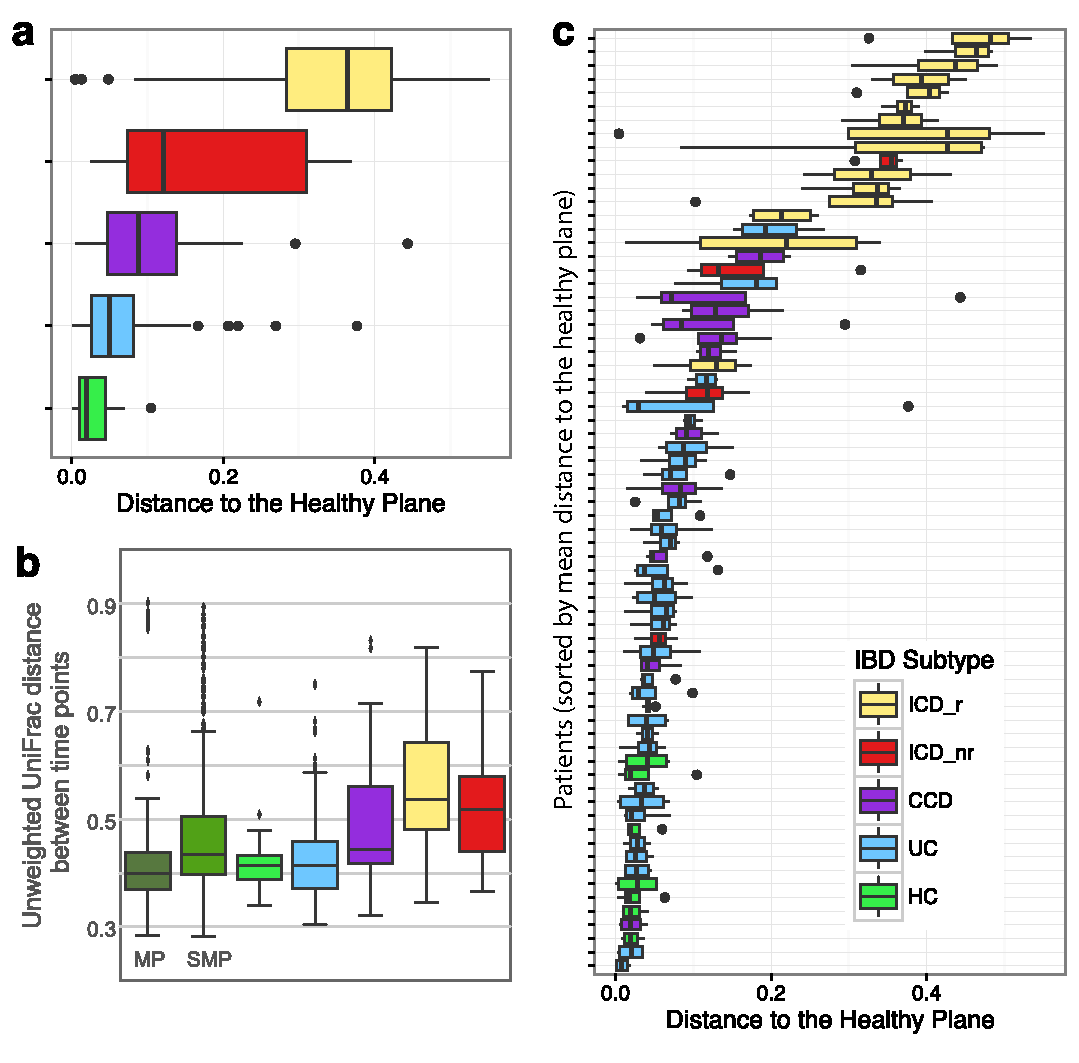
\includegraphics[width=\columnwidth]{plane-figures/Fig2}
\caption[The gut microbiomes of different IBD subtypes display different distributions relative to a healthy plane (HP)]{\textbf{The gut microbiomes of different IBD subtypes display different distributions relative to a healthy plane (HP). a}, Median distances from HP for each IBD subtype. All IBD subtypes were significantly different from healthy controls (GLM, all p $<$ 0.00261). b, UniFrac distances between subsequent samples. c, Distance to HP for each individual patient. HP was defined using data shown in Supplemental~Video 1\textsuperscript{\ref{supVideo2}}. See Supplementary Table~1\textsuperscript{\ref{suppdfFig}} for composition of downstream analysis cohort. Boxes show interquartile range (IQR). Whiskers denote the lowest and highest values within 2.5 × IQR of the median. Circles represent outliers.}
\label{plane-fig2}
\end{figure} 

Although our study represents the largest longitudinal analysis of the \gls{ibd} microbiome to date, the small number of patients in specific subgroups limited some statistical comparisons. Furthermore, the number of healthy controls was lower than the number of \gls{ibd} patients. To address this limitation of unequal sampling of healthy individuals and \gls{ibd} patients, we compared the volatility of our healthy controls to healthy participants in two published studies, the \gls{smp} and the \gls{mp} datasets \cite{RN85,Flores2014}. There was less variability over time in healthy individuals across all three cohorts compared to those with \gls{ibd} (Figure 2b). This result emphasizes that \gls{ibd} is characterized by volatile dysbiosis not found in healthy people, and confirms earlier preliminary results and meta-analysis of much smaller studies \cite{Manichanh2012,Martinez2008,Wills2014,Young2013}.

To extend our understanding of the mechanisms underlying the microbiome dynamics, we explored the correlation between the dynamics and inflammatory activity in each sample using f-calprotectin $>$ 150 $\mu$g/g as a surrogate for inflammatory activity. The concentration of f-calprotectin in stool samples has previously been correlated with endoscopic and histopathologic activity, and is used in daily clinical practice because it is non-invasive \cite{Lewis2011}. We observed that concentrations of f-calprotectin were higher in all \gls{ibd} subtypes than in healthy controls (Figure~\ref{plane-fig3}). However, we did not observe a significant correlation between f-calprotectin and distance from the \gls{hp}  (Figure~\ref{plane-fig3}, \gls{glm} p = 0.275). Although recent microarray analyses of the gut microbiome in a cohort of anti-TNF treated pediatric \gls{ibd} patients\cite{Kolho2015} and experiments with gnotobiotic fecal transplants suggest that microbial composition and function are causally associated with inflammatory activity \cite{Rooks2014}, our differential abundance testing revealed only weak trends and no specific \glspl{otu} that varied significantly with active inflammation, using f-calprotectin $>$ 150 $\mu$g/g as cut-off. However, the use of f-calprotectin as a proxy for inflammatory activity might have introduced bias, because f-calprotectin is a less accurate marker of ileal than colonic inflammation \cite{Sipponen2008} and \gls{icd} patients displayed the greatest distance from the \gls{hp}.

Examples of the microbiome dynamics for one representative \gls{hc} and one from each \gls{ibd} subgroup are shown in addition to changes in f-calprotectin concentrations, distance to \gls{hp}, and Shannon diversity in Figure~\ref{plane-fig4} (all individual profiles are shown in Supplementary Figure~3\footnote{\label{suppdf3}\url{https://images.nature.com/original/nature-assets/nmicrobiol/2017/nmicrobiol20174/extref/nmicrobiol20174-s1.pdf}}), illustrating the more stable dynamics over time for \gls{hc} and \gls{uc} compared to the other clinical phenotypes of \gls{ibd}, with the most fluctuations occurring for patient 69 that had undergone surgical resection. The f-calprotectin levels were low and relatively stable for the \gls{hc} compared to the \gls{ibd} patient (Figure~\ref{plane-fig4}). In these examples, there were also substantial fluctuations in diversity for the \gls{hc}, \gls{icd}-r, and \gls{ccd} by contrast to \gls{uc} and \gls{icd}-nr patients.

\begin{figure}[htbp]
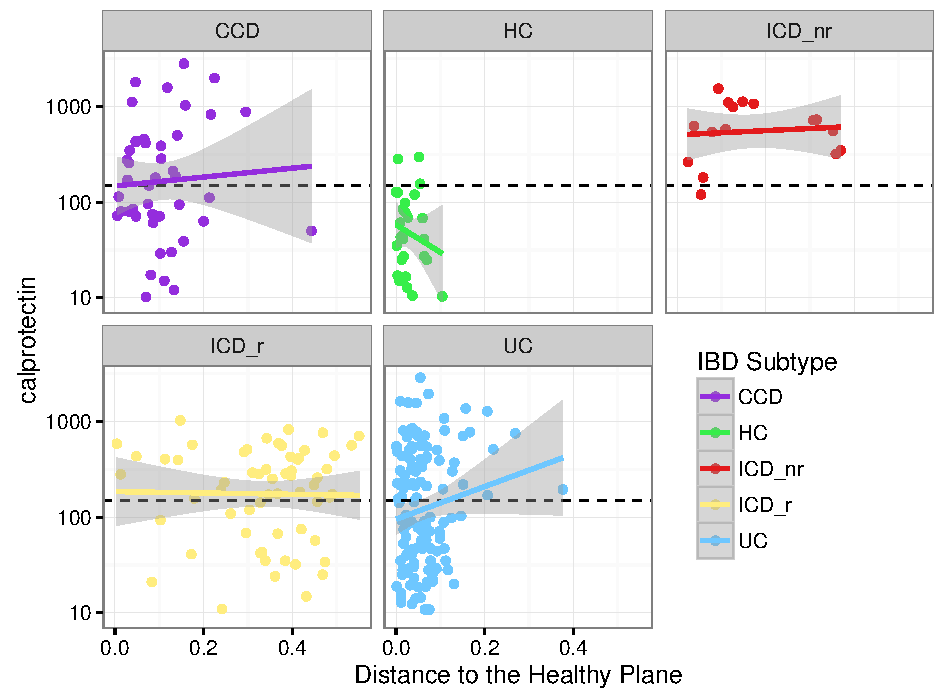
\includegraphics[width=\columnwidth]{plane-figures/Fig3}
\caption[Correlation between fecal calprotectin concentrations and distance to a defined healthy plane (HP) in 3D ordination space.]{\textbf{Correlation between fecal calprotectin concentrations and distance to a defined healthy plane (HP) in 3D ordination space.} Data represent a correlation of f-calprotectin levels and distance to the here defined healthy plane in 3D ordination space (see Supplementary Video~1\textsuperscript{\ref{supVideo2}}) for each individual and time point for different inflammatory bowel disease (IBD) subtypes. To compare the relationship between f-calprotectin and the healthy plane, a generalized linear mixed effects model was fit, with a conditional Gamma distribution, using f-calprotectin and disease type as fixed effects and including a random subject effect; f-calprotectin was not significant (p = 0.27501).}
\label{plane-fig3}
\end{figure} 

\begin{figure}[htbp]
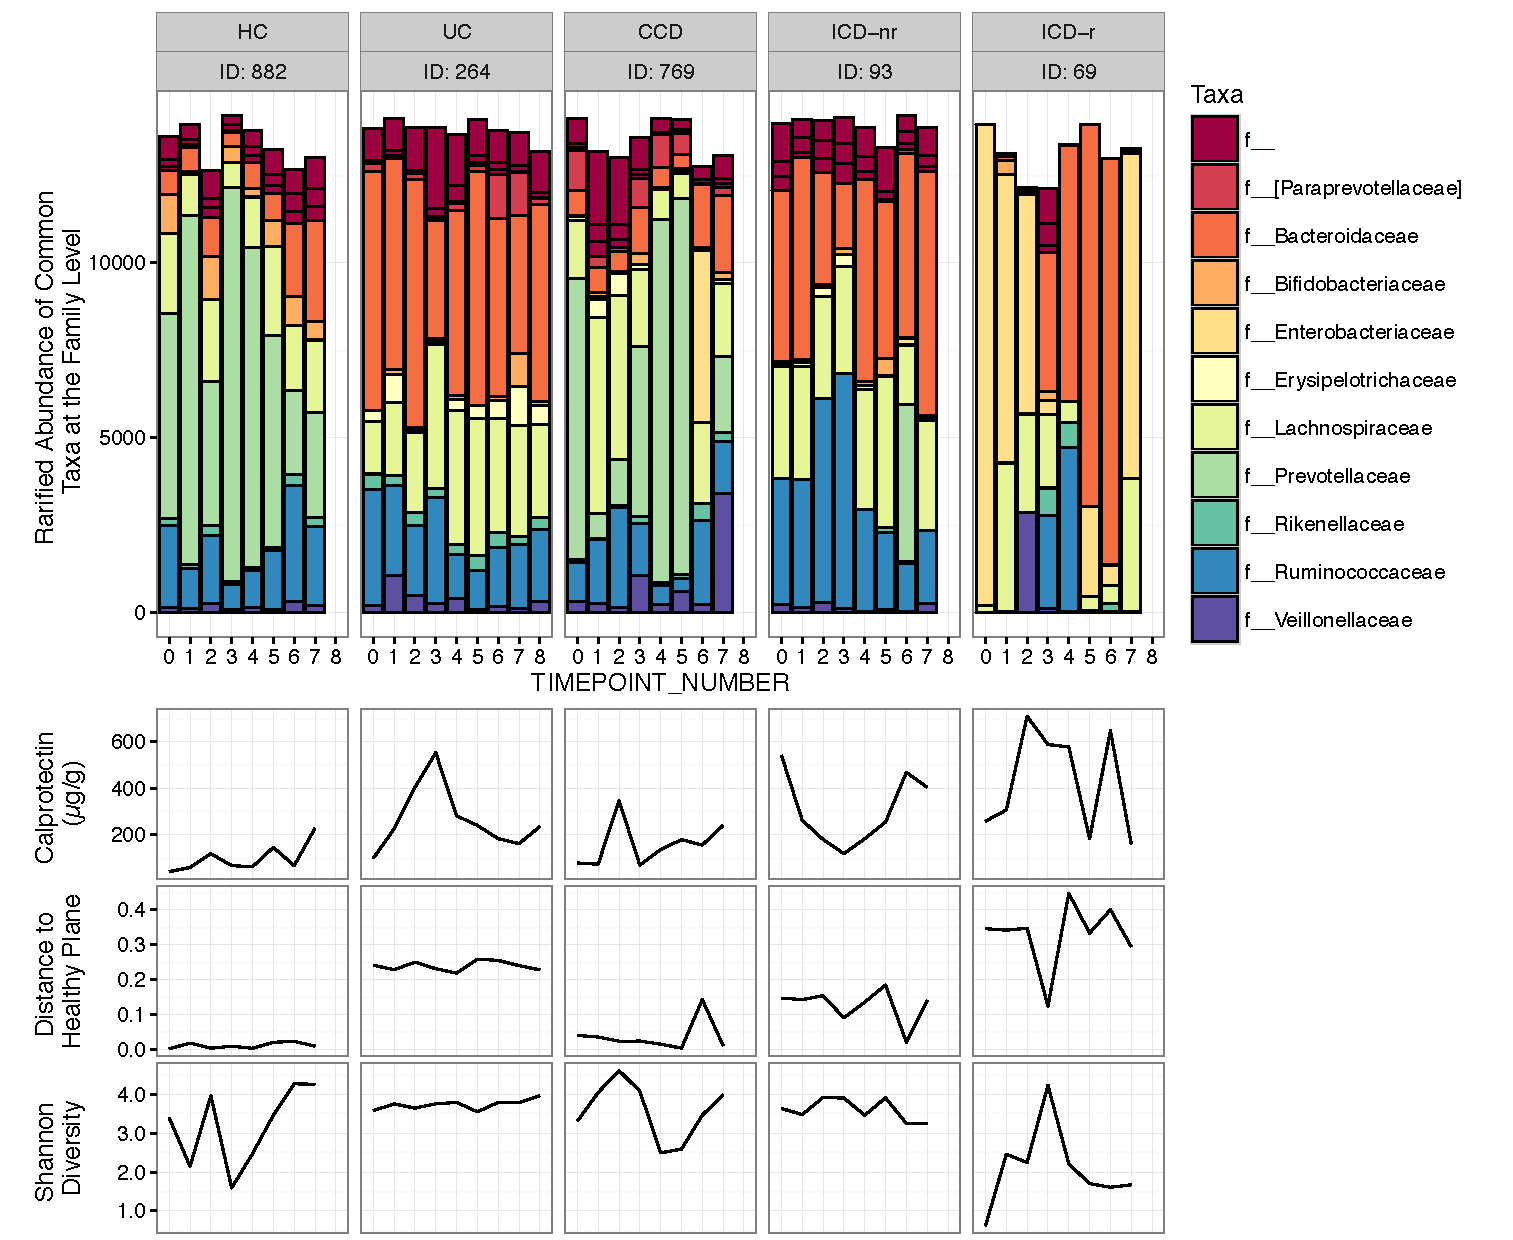
\includegraphics[width=\columnwidth]{plane-figures/Fig4}
\caption[Microbiome dynamics of selected individuals from each IBD subtype and a healthy control.]{\textbf{Microbiome dynamics of selected individuals from each IBD subtype and a healthy control.} From each IBD subtype and healthy control group, representative individuals sampled over the most time points and having complete clinical and sequence data were selected. Data represent f-calprotectin values, distance to the healthy plane, and Shannon diversity and rarified abundances of most common taxa at the family level. Note that taxa unclassified at the family level are represented in the ‘f\textunderscore' category.}
\label{plane-fig4}
\end{figure} 

We further explored the individual dynamics of the gut microbiome in \gls{ibd} patients who experienced increased clinical disease activity, according to the physician's global assessment (Supplementary Figure~4\textsuperscript{\ref{suppdf3}}). Recently, the short-term (6 weeks) dynamics of the microbiome in pediatric patients with active \gls{ibd} treated with anti-TNF indicated that initiation of medical treatment changes the microbial composition at the genus level \cite{Kolho2015}. Because we had few anti-TNF exposed patients, and our patients received a course of corticosteroids at flare as first line therapy, we explored how corticosteroid administration influenced microbiome dynamics. Our data demonstrate that change in medication influenced the volatility of the microbiome (Supplementary Figure~4\footnote{\url{https://images.nature.com/original/nature-assets/nmicrobiol/2017/nmicrobiol20174/extref/nmicrobiol20174-s1.pdf}}). Patients receiving a course of oral corticosteroids (n=7) had more microbiome fluctuations than patients on stable medication (n=49), based on calculations of unweighted UniFrac distance between time points (Wilcoxon Signed-rank test; p=0.04). Our dynamic model suggests that beyond the association with \gls{ibd} subtype and the weak correlation with inflammation, the dynamics of the microbiome composition are influenced by changes in medication. The extent to which other factors, such as dietary changes and smoking, may have influenced the observed volatility remains speculative, because the collected information was insufficiently detailed to include these factors as covariates.

To evaluate the microbiome as a predictive tool, we combined the microbial and clinical data and used a supervised learning Random Forests model to predict \gls{ibd} subtypes \cite{RN4205,Love2014}. To avoid overfitting, our models were built using \gls{otu} abundances from the first time points only, along with clinical metadata (\gls{bmi}, f-calprotectin concentrations, sex, and Distance to the \gls{hp}). Accuracy was evaluated using the remaining three time points, which were not used to train the model. Using this model, the \gls{ibd} subtypes were discriminated from healthy controls and correctly predicted for 66.6\% of samples (Supplementary Table~2\footnote{\label{suppdf4}\url{https://images.nature.com/original/nature-assets/nmicrobiol/2017/nmicrobiol20174/extref/nmicrobiol20174-s1.pdf}}), consistent with the findings reported in Gevers et al. (2014). Feature importance scores from this model revealed several potential microbial indicators of \gls{ibd} subtypes, including \glspl{otu} matching to \textit{Lachnospira}, \textit{Clostridium}, \textit{Oscillospira}, and many unidentified \textit{Ruminococcaceae} (Supplementary Table~3\textsuperscript{\ref{suppdf4}}). Intriguingly, the accuracy of the model increased slightly if f-calprotectin concentrations were omitted, but decreased by at least 10\% if the distance to the \gls{hp} was removed (Supplementary Tables 2 and 3\textsuperscript{\ref{suppdf4}}), suggesting that the \gls{hp} is a more important factor in the model. Comparable levels of accuracy were previously achieved using rectal samples \cite{Gevers2014}, but here we show that the same can be achieved with fecal samples, which are easier to collect. When immunochip data were included for a subset of 29 \gls{ibd} individuals and the Random Forests model was repeated, the samples were still classified into the four \gls{ibd} subtypes (\gls{uc}, \gls{ccd}, \gls{icd}-r, \gls{icd}-nr) (Supplementary Tables 2 and 3\textsuperscript{\ref{suppdf4}}). While distance to the \gls{hp} remained as the single most important feature for classification,\gls{gls} were more predictive than sex, f-calprotectin, or \gls{bmi} when included in the model (Supplementary Table~2\textsuperscript{\ref{suppdf4}}). However, including \gls{gls} only increased the overall accuracy of the model by about 2\%, demonstrating the predictive potential of the microbiome. Interestingly, in a recent study of obesity covering 339,224 individuals, the 97 risk loci for obesity accounted for only 2.7\% of \gls{bmi} variation \cite{Locke2015}, whereas the microbiome classified lean from obese individuals with 90\% accuracy \cite{Knights2011}, providing precedent for the predictive value of the gut microbiome over human genetics in chronic disease.

In summary, by analyzing fecal samples collected every 3 months from a large \gls{ibd} cohort, we determined the long-term volatility of the gut microbiome in \gls{ibd}. Our data revealed that although the microbiome of healthy individuals varied it was only within a newly defined \gls{hp}, whereas there was considerable volatility away from the \gls{hp} for several of the \gls{ibd} cohorts. Devising improved methods to detect the healthy state with non-invasive sampling, to predict when the healthy state will be departed, and to sustain the microbiome in this healthy state by erecting barriers that prevent the slip back into dysbiosis, will be an important focus of future work.


\subsection{Methods}

\subsubsection{Cohort Demographics}

Patients with \gls{cd} or \gls{uc}, the two major forms of \gls{ibd}, attending the outpatient clinic were consecutively invited to take part. After obtaining written consent, \gls{bmi} was recorded and patients were asked to provide a fecal sample and to fill in a questionnaire with clinical disease activity, present medication, dietary habits, use of antibiotics and use of \glspl{nsaid}. Disease phenotype was classified according to the Montreal classification \cite{Silverberg2005}. Individuals were then followed prospectively, asked to provide fecal samples and to fill in the questionnaire every third month for a two-year period. If a patient did not provide a fecal sample at any of the three months periods, a reminder letter was sent. In total 109 patients with \gls{ibd} (\gls{cd}; n=49 and \gls{uc}; n=60) took part. Nine additional individuals with no \gls{ibd} or any other gastrointestinal conditions were recruited as \gls{hc} as well as 19 patients with other chronic inflammatory gastrointestinal diseases (4 \gls{lc} and 15 \gls{cc}).  All 137 individuals were Caucasians and together they provided 683 fecal samples during the two-year period (Supplementary Table~4\footnote{\url{https://images.nature.com/original/nature-assets/nmicrobiol/2017/nmicrobiol20174/extref/nmicrobiol20174-s1.pdf}}). The study was approved by the Ethical Committee of the Medical Faculty, Uppsala University (2007/291).

\subsubsection{Sample Collection}

Fecal samples were self-collected in sterile plastic containers and stored at -80 °C until shipping on dry ice and processing.

\subsubsection{Fecal calprotectin} 

To assess the degree of inflammatory activity at the collection of each fecal sample, the concentration of f-calprotectin was assessed by commercially available ELISA, Calprotectin Elisa Buhlmann Laboratories AG, Basel, Switzerland, according to the manufacturer's protocol. 

\subsubsection{DNA Extraction and Amplification}

Genomic DNA was extracted from 0.25 g of fecal material from each sample using the Earth Microbiome DNA extraction protocol \cite{EMP2011}. Briefly, DNA was extracted using the 96-well format MoBio Powersoil DNA kit on an EpMotion 5075 robot with vacuum (Eppendorf, Hamburg, Germany). DNA was quantified with the Qubit 2.0 fluorometer (Invitrogen, Carlsbad, CA) according to the manufacturer's instructions.

PCR amplification and library preparation were performed similarly to the protocol described by Caporaso et al. \cite{Caporaso2011proceedings}. 515F/806R Illumina primers with unique reverse primer barcodes were used to target the V4 region of the 16S rRNA gene. Samples were amplified in triplicate and cleaned using the MO BIO 69 htp PCR cleanup kit. Each PCR reaction included 1X PCR buffer, 10 $\mu$M each forward and reverse primer, 200 μM dNTPs, 1 U/ml Taq polymerase, 15 ng template DNA, and PCR grade water, with a total reaction volume of 25 $\mu$L. Reactions were kept at 94\textdegree C for 3 minutes for denaturation to occur. Amplification was performed by 25 cycles of 94\textdegree C for 45s, 58\textdegree C for 60s, and 72\textdegree C for 90s. The V4 amplicons were sequenced on the Illumina HiSeq 2000 platform, yielding single end, 100 base pair reads. Sequencing and quality assessment were performed at the Yale Center for Genome Analysis.

\subsubsection{Phylogenetic Analysis}

Sequence data were processed using QIIME 1.9.0-dev through the online platform QIITA\footnote{\url{https://qiita.ucsd.edu}}\cite{RN110}. Four HiSeq lanes of data were demultiplexed with default quality filtering settings and subsequently combined, resulting in 248,547,926 total sequences. These sequences were clustered using SortMeRNA at 97\% identity against the Greengenes rRNA reference database May 2013 release \cite{Kopylova2012,McDonald2012}. Sequences that failed to match the database were discarded. 237,653,256, or approximately 95.6\% of the sequences, clustered against the Greengenes reference dataset. Even sampling was performed at 14,553 sequences per sample for beta diversity and supervised learning analyses. The beta diversity principal coordinates plot of unweighted UniFrac distances was constructed using the same rarefied \gls{otu} table, and visualized in Emperor \cite{Lozupone2005,Vazquez2013}. Clinical matched metadata, including f-calprotectin concentrations, were included when available. From each patient, the first four microbiome samples with matched f-calprotectin concentrations were sub-selected for use in downstream analysis. 

\subsubsection{Statistical Analysis.}

The R package phyloseq was used to import and graph data, while the packages DESeq2, randomForest, and vegan were used to perform differential abundance testing and supervised learning \cite{Ihaka1996,Liaw2002,Love2014,McMurdie2013,Oksanen2016}. Statistical significance of unweighted UniFrac distance matrices comparing healthy controls and \gls{ibd} subtypes was assessed using the ADONIS test. The variation of the microbial community over time was calculated with vector lengths produced by summing the total distance between each subject's time points over the first three \gls{pcoa} axes of unweighted UniFrac space. The Random Forests model was constructed using the first time point from each patient in the downstream analysis cohort and prediction accuracy was measured using the subsequent three time points  (\gls{ccd} = 11 patients, \gls{icd} without resection (\gls{icd}-nr) = 4 patients, \gls{icd} with resection (\gls{icd}-r) = 15 patients, \gls{uc} = 30 patients, and \gls{hc} = 7 patients). The following metadata categories used as features for supervised learning: \gls{bmi}, f-calprotectin (continuous), sex, and Distance to the Healthy Plane. For classification on the subset of samples with immunochip data, the above process was used while adding \gls{gls}. We used a dataset of 29 \gls{ibd} samples (25 \gls{cd}, 4 \gls{uc}) with available immunochip data to estimate a \gls{gls} for each sample. In particular, \gls{gls} was calculated summing the number (counts) of risk alleles (0,1,2) at lead \gls{snp} from each \gls{ibd} risk locus (n = 163) according to Jostins et al. \cite{Jostins2012}.

After performing principal coordinates analysis of the unweighted UniFrac distance matrix, the samples of \gls{hc} were used to fit using the least squares method on the first three principal coordinates. The distance from each sample to this plane was measured and added to the sample metadata both for weighted and unweighted UniFrac. To compare distribution of samples relative to this healthy plane, a generalized linear mixed effects model was fit, with a conditional Gamma distribution, using disease type as a fixed effect and including a random subject effect.

To assess the variation between samples in an orderly manner (as described by the time point), we measured the UniFrac (weighted and unweighted) distance between samples that occur sequentially for any given subject; samples representing the final collection point do not have a value in these columns, as there is no subsequent sample to compare to.

We examined the power of differential abundance tests for the 16S data. DESeq2 \cite{Love2014} assumes that counts can be modeled as a negative binomial distribution with a mean parameter, allowing for size factors, and a dispersion parameter. The test for differential abundances fits a generalized linear model with a negative binomial family and a log link function. 

A power analysis was conducted by using samples from the downstream analysis cohort (Supplementary Table~4\footnote{\url{https://images.nature.com/original/nature-assets/nmicrobiol/2017/nmicrobiol20174/extref/nmicrobiol20174-s1.pdf}}). The power of the differential abundance test is dependent on the sample size of groups, difference in mean counts, type 1 error rate, and the dispersion value. Here we used a conventional type 1 error rate of 0.05 and assumed that we have two groups with sample sizes of n1 = 25 and n2 = 80. A total of 1000 \glspl{otu} were randomly selected from the data and dispersion parameters were estimated for each \gls{otu}. Data was then simulated from a negative binomial distribution, as specified by DESeq2, for each estimated dispersion value with means giving 2 fold, 1.5 fold, and 1.25 fold differences. For each mean fold difference value and dispersion value, a total of 5000 data simulations were done and a Wald test for difference in means using a generalized linear model was conducted. Based on these simulations, where data is generated with true differences, the fraction of times that the null hypothesis is correctly rejected (the power), was calculated and our comparisons were well powered given our subset sample sizes (Supplementary  Table~4\footnote{\url{https://images.nature.com/original/nature-assets/nmicrobiol/2017/nmicrobiol20174/extref/nmicrobiol20174-s1.pdf}}). 

\textbf{Data Availability:} Microbiome data from this study is available on Qiita under study ID 1629 (https://qiita.ucsd.edu/study/description/1629) and using the EBI accession number ERP020401. Patient clinical information is available on Qiita and in Supplemental Dataset~1\footnote{\url{https://images.nature.com/original/nature-assets/nmicrobiol/2017/nmicrobiol20174/extref/nmicrobiol20174-s2.txt}}. 

\textbf{Code Availability:} Our analysis methods make use of standard, open source software. R software packages are available on CRAN\footnote{\url{cran.r-project.org}}, bioconductor\footnote{\url{bioconductor.org}}, and GitHub\footnote{\url{github.com/joey711/phyloseq}}. Python software is available in the bioconda and biocore Conda channels, and is maintain on GitHub\footnote{\url{github.com/biocore, github.com/ElDeveloper/reference-plane}}.
